\chapter{Standard and Extended Form Games}
\label{cha:game-theory}

\mpic{gametheory/neumann}{John Von Neumann}{1903}{1957}{Pioneer of the
  digital computer, game theory and cellular automata.}  In all
multiagent systems we have a set of autonomous agents each performing
its own actions using whatever information is has available. Since the
other agents are also taking actions, each agent must also take these
into account when deciding what to do. Thus, what one does depends on
what the other one does and vice-versa. The agent must decide what to
do when their choice of action depends on the others' choices. These
types of problems are very common in different fields, from Economics
to Biology, and their solution is sometimes of immense importance. As
such, a set of mathematical tools has been developed over the years to
model and solve these problems. It is known as \td{game theory} and is
the subject of this and several other chapters in this book.

Game theory was first formally introduced in the book \emph{``The
  Theory of Games and Economic Behavior''} \cite{neumann44a}. The book
introduced a mathematical way of analyzing certain types of decisions
where two or more parties take actions that impact all. In this
chapter we present the two most basic forms of games: normal and
extended form games.  These games are known as \td{non-cooperative
  games} because the agents' preferred sets of actions can be in
conflict with each other.  That is, what is good for one agent might
be bad for the others. Of course, the fact that they can be in
conflict does not mean that they have to be, thus, non-cooperative
games can lead to cooperation.

\section{Games in Normal Form}
\label{sec:normal-form}

%\mc{For a more complete introduction to game theory read
%  \cite{osborne04a}.} 
In the simplest type of game we have two agents each of which must
take one of two possible actions. The agents take their actions at the
same time. They will then each receive a utility value, or payoff,
based on their joint actions. Games such as this one can be
represented using a \td{payoff matrix} which shows the utility the
agents will receive given their actions.  Figure~\ref{fig:stanform}
shows a sample game matrix in \td{normal form}, also known as
\td{strategic form}, a phrase introduced by Shapley in 1965.  In this
game if Bob takes action $a$ and Alice takes action $c$ then Bob will
receive a utility of 1 and Alice a utility of 2. We can extend the
payoff matrix to any number of players and actions. In these games we
always assume that the players take their actions simultaneously.

\begin{SCfigure}
  \begin{minipage}{1.0\linewidth}
    \begin{center}
      \renewcommand\arraystretch{1.5}
      \begin{tabular}{cc|c|c|}
        &    &\multicolumn{2}{c}{Alice} \\ 
        &      &$c$&$d$ \\ \cline{1-4}
        \multirow{2}{2em}{Bob}
        & $a$  &1,2 &4,3 \\ \cline{2-4}
        & $b$  &3,2 &2,4 \\ \cline{2-4}
      \end{tabular}
    \end{center}
    \caption{Sample game matrix in normal form.}
    \label{fig:stanform}
  \end{minipage}
\end{SCfigure}

Normal form games also assume that the players have \td{common
  knowledge} of the utilities that all players can receive. That is,
everybody knows that everybody knows that everybody knows, and so on,
the values in the payoff matrix. \mc{\cite{reasoning:about:knowledge}
  describes a logic for representing agents' knowledge about others'
  knowledge.}  This situation is different from having the agents know
the values in the matrix but not know that the others know those
values. For example, if you know that I am giving you a surprise party
then you might go along and act surprised when we all jump and yell
``surprise!''. However, if you know that I know that you know that I
will be giving you a surprise party then the deception will no longer
work.

It is also interesting to note that in message-passing multiagent
systems where messages can be lost it is impossible for agents to ever
achieve common knowledge about anything
\cite{reasoning:about:knowledge}. The problem is historically
described as the \td{Byzantine generals problem} where two generals
from the same army are poised on opposite sides of a valley which is
occupied by the enemy. The generals must both attack at the same time
in order to defeat the enemy. However, their only method of
communication is by sending a messenger who could be captured by the
enemy. We can see that, if one general sends a message to the other
saying ``We attack at dawn'' it has no way of confirming whether the
other general received this message. Similarly, if a general does
receive the message and sends another messenger back acknowledging
receipt then it has no way of confirming whether the other general
received the acknowledgment. Thus, it is impossible to agree on a
time. In practice, however, multiagent systems that need common
knowledge either give their agents this common knowledge from the
beginning or assume that communications are reliable enough that it is
safe to assume that all messages are delivered.

Getting back to the normal form game, we define a \td{strategy} $s$ to
be the set of actions all players take. In this case a strategy of $s
= (a,c)$ would give Bob a utility of 1 and Alice a utility of 2, in
other words, $u_{\text{Bob}}(s) = 1$ and $u_{\text{Alice}}(s) = 2$.
We also refer to Bob's strategy in $s$ as $s_{\text{Bob}}$, which is
$a$ in this case. This strategy is also an example of a \td{pure
  strategy}: one where the agents take a specific action. In contrast,
a \td{mixed strategy} is one where the agents take different actions,
each with some fixed probabilities. For example, a mixed strategy for
Bob is to take action $a$ with probability of .3 and action $b$ with a
probability of .7. Note that in a mixed strategy the probabilities for
all actions of each agent have to add up to 1. Typically, game theory
further assumes that players are \td{rational}, which we use as a
synonym for selfish. That is, a rational player always acts so as to
maximize its utility.

A special type of game are those in which the values in every box of
the matrix add up to zero. These games are known as \td{zero-sum}
games and represent scenarios where one agent's gain must come at a
loss to he other agents. For example, in a zero-sum game with two
players if for a particular strategy $s$ one player gets a utility of
5 then the other player must receive a utility of $-5$.  In these
games cooperation is unlikely. Note that every competitive sport is a
zero-sum game as the fact that one team wins means the other must
lose.  Luckily, real-world problems are rarely zero-sum, even if our
tendency is often to perceive them as such.

%  \begin{itemize}
%  \item  Players are \emph{rational} (selfish). Participation is
%    better than not.
%  \item Strategy $s$ is \emph{stable} if no agent is motivated to
%    diverge from it.
%  \item A game is \emph{zero-sum} if the sum of payoffs for every
%    $s$ is 0.
%  \end{itemize}
%In a zero-sum game one player's gain is, by definition, the other
%players' loss, exactly. I have heard people who mistakenly use this
%term to mean that all choices for a player have their drawbacks (and
%are, in a way, the same). For example:

%\begin{quotation}
%``Also, Healy said, the programs pushed up sales earlier this summer
%  at the expense of later sales, causing a `zero-sum game.' ''
%  --\hreffoot{http://www.newsday.com/business/ny-bzgm4398003aug26,0,6021111.story?coll=ny-business-headlines}{Newsday.com 8/26/05}.}
%\end{quotation}

%If all choices have the same payoff for an agent then all the numbers
%will be the same \emph{for that agent}. In the quote above there is no
%other agent involved. What Healy is trying to say is that both
%programs are equivalent (or have equivalent payoffs).

\subsection{Solution Concepts}

Given a game matrix we can't help but ask: what strategy should they
use? Which is best the best strategy in any given game? The problem,
of course, is that there is no simple way to define what's best since
what is best for one agent might not be good for another. As such,
different solution concepts have been proposed.

The earliest solution concepts were proposed by Von Neumann. He
realized that in any given game an agent could always take the action
which maximized the worst possible utility it could get. This is known
as the \td{maxmin strategy}, or minmax, if we are talking about losses
instead of gains. Specifically, in a game with two agents, $i$ and
$j$, agent $i$'s maxmin strategy is given by
\begin{equation}
  \label{eq:maxmin}
  s_i^* = \max_{s_i} \min_{s_j} u_i(s_i,s_j).
\end{equation}

That is, $i$ assumes that no matter what it does $j$ will take the
action that is worst for $i$. Thus, $i$ takes its best possible action
given this assumption. Unfortunately, the strategy where both players
play their maxmin strategy might not be stable in the general case. In
some payoff matrices it can happen that if $i$ knows that $j$ will
play its maxmin strategy then $i$ will prefer a strategy different
from its maxmin strategy. For example, in figure~\ref{fig:stanform}
the maxmin strategy is $(b,d)$ but if Alice plays $d$ then Bob should
play $a$. Thus, that strategy is not stable. This problem has
prevented the maxmin strategy from becoming a popular solution
concept.

The existence of a solution concept is also important to us since, if
a solution concept does not exist for the game we are interested in
then it is not of any use to us. For the maxmin strategy we have the
\td{minimax theorem} which states that a strategy that minimizes the
maximum loss, a minmax strategy, can always be found for all
two-person zero-sum games \cite{neumann28a}. Thus, we know it will
work at least for this subset of games.

Another approach is to look for strategies that are clearly better. We
say that $s$ is the \td{dominant} strategy for agent $i$ if the agent
is better off doing $s$ regardless of which strategies the others use.
Formally, we say that a pure strategy $s_i$ is dominant for agent $i$ if
\begin{equation}
  \label{eq:dominant}
  \forall_{s_{-i}} \forall_{r_i \neq s_i} u_i(s_{-i}, s_{i})
  \geq u_i(s_{-i}, r_i),
\end{equation}
where $s_{-i}$ represents the strategies of all agents except $i$.
This idea can be expanded into the \td{iterated dominance} solution in
which dominated strategies are eliminated in succession. First we
eliminate strategies from one agent, then from another, and so on in a
round-robin manner (and repeating agents) until we check all agents in
successions and none has a dominated action. Unfortunately, the
iterated dominance algorithm almost always ends before a solution is
found. That is, in most games none of the players has a dominant
strategy.

We can also take a step back and look at the problem from a system
designer's perspective. With our new enlightened outlook we might
think that the right solution is to maximize overall welfare for all
players. The \td{social welfare} strategy is the one that maximizes
the sum of everyone's payoffs. That is
\begin{equation}
  \label{eq:social-welfare}
  s^* = \arg \max_s \sum_i u_i(s).
\end{equation}

However, once again we have the problem that a social welfare strategy
might not be stable. Each selfish agent cares only about his own
utility and will thus play a different strategy if it can get a higher
utility, even if it means everyone else is much worse. Also, the
social welfare strategy might not seem fair as it could be one where
one agent gets an extremely high utility and everyone else gets
almost nothing.

We can solve the unfairness problem by defining a solution concept
that does not take into account the agents' absolute utility values.
\mpic{gametheory/pareto2}{Vilfredo Pareto}{1848}{1923}{} A strategy
$s$ is said to be \td{Pareto optimal} if there is no other strategy
$s'$ such that at least one agent is better off in $s'$ and no agent
is worse off in $s'$ than in $s$. There can be more than one Pareto
optimal solutions for a given problem. The set of all Pareto
strategies for a given problem is formally defined to be the set
\begin{equation}
  \label{eq:pareto-soln}
\{s \,|\, \neg \exists_{s' \neq s} (\exists_{i} u_i(s') >
    u_i(s) \wedge \neg \exists_{j \in {-i}} u_j(s) > u_j(s'))\}
\end{equation}
where $-i$ represents the set of all agents except $i$. Pareto
solutions are highly desirable from a social welfare perspective as
they ensure that no one agent can complain that it could get more
utility without hurting someone else in the process. In Economics the
Pareto solution of often referred to as Pareto efficient or, simply,
the \td{efficient} solution. Unfortunately, Pareto solutions might
also be unstable in that one player might have an incentive to play a
different action because he gets higher utility, which means others
get lower utility. In a dynamic multiagent system stability can be
very important as designers often want the system to converge.

The problem of lack of stability was solved by John F. Nash. We say
that a strategy $s$ is a \td{Nash equilibrium} if for all agents $i$,
$s_i$ is $i$'s best strategy given that all the other players will
play the strategies in $s$. That is, if everyone else is playing the
Nash equilibrium then the best thing for everyone to do is to play the
Nash equilibrium. As with the Pareto solution, a game can have more
than one Nash equilibrium. Formally, the set of all Nash equilibrium
strategies for a given game is given by
\begin{equation}
  \label{eq:nash-eq}
    \{s \,|\, \forall_{i} \forall_{a_i \neq s_i} u_i(s_{-i}, s_i) \geq
    u_i(s_{-i}, a_i) \}.
\end{equation}

Nash showed that all game matrices have at least one equilibrium
strategy, but this strategy might be mixed. The only problem with the
Nash equilibrium is the fact that in many games there are many such
equilibria. Also, some of those Nash equilibria might be better for
some players than other. Thus, the players might end up arguing about
which specific one to adopt. Still, once the agents have agreed on one
it is a very stable solution. Note that there is no general relation
between the Nash equilibrium and the Pareto solution. That is, a
strategy can be a Nash equilibrium but not be a Pareto solution.
Similarly, a strategy can be Pareto optimal but not be a Nash
equilibrium. On the other hand, the social welfare strategy must be a
Pareto optimal.\mpic{gametheory/nash}{John F.  Nash}{1928}{}{Winner of
  1994 Nobel prize on Economics.}

\medskip

All these solution concepts make it clear that it is not a simple
matter to define what is the best answer. With multiple players, what
is best depends on how much we are willing to respect the agents'
selfishness, how we trade-off the various agents utilities, and how
fair we wish to be.

The most common problem we face when designing multiagent systems is
the existence of multiple equilibria. That is, we can generally design
a system so that selfish agents will converge to an equilibrium
solution if there is one. But, if there are more than one solution
then we need to add extra coordination mechanisms to ensure that the
agents converge to the same strategy.

\subsection{Famous Games}

\begin{SCfigure}
  \begin{minipage}{1.0\linewidth}
    \begin{center}
    \renewcommand\arraystretch{1.5}
  \begin{tabular}{cc|c|c|}
&    &\multicolumn{2}{c}{A} \\ 
&      &Stays Silent&Betrays \\ \cline{1-4}
\multirow{2}{2em}{B}
& Stays Silent  &\parbox{8em}{\raggedright \vspace{1em}Both serve six months.\vspace{1em}}&\parbox{8em}{\raggedright B serves 10 years; A goes free.} \\ \cline{2-4}
& Betrays  &\parbox{8em}{\raggedright \vspace{1em}A serves 10 years; B goes free.\vspace{1em}}&\parbox{8em}{\raggedright Both serve two years.} \\ \cline{2-4}
\end{tabular}
    \end{center}
  \end{minipage}
  \caption{Payoff matrix for original prisoner's dilemma problem.}
  \label{fig:orig-pd}
\end{SCfigure}

The most famous game of all is the \td{Prisoner's Dilemma}. Its story
typically goes something like the following.
\begin{quotation}
    Two suspects A, B are arrested by the police. The police have
    insufficient evidence for a conviction, and having separated both
    prisoners, visit each of them and offer the same deal: if one
    testifies for the prosecution against the other and the other
    remains silent, the silent accomplice receives the full 10-year
    sentence and the betrayer goes free. If both stay silent, the
    police can only give both prisoners 6 months for a minor charge.
    If both betray each other, they receive a 2-year sentence each.
\end{quotation}

From this story we can generate a payoff matrix as shown in
figure~\ref{fig:orig-pd}. We can replace the prison sentences with
utility values and arrive at the standard prisoner's dilemma payoff
matrix shown in figure~\ref{fig:pd}, note that longer prison terms
translate into lower utility. Thus, a 10 year sentence gets a utility
of 0, a 2 year sentence has utility of 1, 6 months is 3, and no time
served has utility of 5. The actions are labeled cooperate and defect
because the suspects can either cooperate with each other and maintain
their silence or defect from their coalition and tell on the other
one.

\begin{SCfigure}
  \begin{minipage}{1.0\linewidth}
    \begin{center}
      \renewcommand\arraystretch{1.5}
      \begin{tabular}{cc|c|c|}
        &    &\multicolumn{2}{c}{A} \\ 
        &      &Cooperate&Defect \\ \cline{1-4}
        \multirow{2}{2em}{B}
        & Cooperate  &3,3 & 0,5 \\ \cline{2-4}
        & Defect  &5,0 &1,1 \\ \cline{2-4}
      \end{tabular}
    \end{center}  
    \end{minipage}
  \caption{Prisoner's dilemma with standard payoff values.}
  \label{fig:pd}
\end{SCfigure}


Analysis of this matrix reveals that the social welfare solution is
(C,C), the set of Pareto optimal strategies is \{(C,C) (D,C) (C,D)\},
the dominant strategy for both players is Defection, and the Nash
equilibrium strategy is (D,D).
  
The Prisoner's dilemma is interesting because the best choice is not
the rational choice. That is, even thought the (C,C) solution Pareto
dominates the (D,D) solution, a rational player will only play D as
that strategy is dominant. The game is widely studied because it
applies to many real-world situations like nuclear disarmament and
getting kids to clean up their room. There are some that object to the
fact that defection is the equilibrium and claim that real people do
not act like that.

\begin{SCfigure}
  \begin{minipage}{1.0\linewidth}
    \begin{center}
      \renewcommand\arraystretch{1.5}
      \begin{tabular}{cc|c|c|}
        &    &\multicolumn{2}{c}{Alice} \\ 
        &      &Ice Hockey&Football \\ \cline{1-4}
        \multirow{2}{2em}{Bob}
        & Ice Hockey  &4,7 & 0,0 \\ \cline{2-4}
        & Football  &3,3 & 7,4 \\ \cline{2-4}
      \end{tabular}
    \end{center}
  \end{minipage}
  \caption{Battle of the sexes game.}
  \label{fig:battlesex}
\end{SCfigure}


\medskip The \td{battle of the sexes} is another popular game. It is
shown in figure~\ref{fig:battlesex}. In this game Alice and Bob like
each other and would like to spend time together but must decide,
without communicating with each other, where to go. Alice likes ice
hockey while Bob likes football. As such, they have a
\idx{coordination problem} where each prefers to go to a different
place but they would like to be together. This type of problem arises
frequently in multiagent systems where we often have agents that want
to cooperate with each other to achieve some larger goal but have
conflicting priorities about how to achieve that goal.  For example,
the agents in a company want to get a new contract so that they can
all get paid but each one wants to do as little work as possible while
getting as much money as possible. Another example is agents that want
to deliver a package but have different preferences on where the
hand-off from one agent to the other should occur.

After some analysis of this game we can determine that the social
welfare solutions are (I,I) (F,F), the Pareto optimal solutions are
also (I,I) (F,F), there is no dominant strategy, and the Nash
equilibrium solutions are (I,I) (F,F). As you can see, the problem
here is that there are two strategies both of which are equally
attractive. This is the type of problem that we could fix easily if we
just had a little communication.

\medskip
\begin{SCfigure}
  \begin{minipage}{1.0\linewidth}
    \begin{center}
    \renewcommand\arraystretch{1.5}
  \begin{tabular}{cc|c|c|}
&    &\multicolumn{2}{c}{Alice} \\ 
&      &Continue&Swerve \\ \cline{1-4}
\multirow{2}{2em}{Bob}
& Continue  &-1,-1 & 5,1 \\ \cline{2-4}
& Swerve  &1,5 & 1,1 \\ \cline{2-4}
\end{tabular}
  \end{center}
  \end{minipage}
  \caption{The game of chicken.}
  \label{chicken}
\end{SCfigure}

The \td{game of chicken}, shown in figure~\ref{chicken}, is also
common.  In this story, two maladjusted teenagers drive their cars
towards each other at high speed. The one who swerves first is a
chicken and thus loses the game. But, if neither of them swerves then
they both die in a horrible crash. After some analysis we can see that
this game is very similar to the battle of the sexes. Its social
welfare, Pareto optimal, and Nash strategies are all the same, namely
(C,S) (S,C), and there is no dominant strategy. Once again there is a
coordination problem: who will be the chicken?

One way out of the problem of multiple Nash equilibria is for one of
the players to eliminate one of his choices, say by soldering the
steering wheel of the car so that it does not turn. This would make it
so that the other player's rational choice is to swerve. It might seem
counter intuitive but in cases like this an agent can increase its
payoff by limiting its set of possible actions.  

\medskip

\begin{SCfigure}
  \begin{minipage}{1.0\linewidth}
    \begin{center}
    \renewcommand\arraystretch{1.5}
  \begin{tabular}{cc|c|c|}
&    &\multicolumn{2}{c}{Pig} \\ 
&      &Nothing&Press Lever \\ \cline{1-4}
\multirow{2}{2em}{Piglet}
& Nothing  &0,0 & 5,1 \\ \cline{2-4}
& Press Lever  &-1,6 & 1,5 \\ \cline{2-4}
\end{tabular}
  \end{center}
  \end{minipage}
  \caption{The pig and the piglet.}
  \label{fig:piglet}
\end{SCfigure}

The final game is taken from the world of zoology.  Imagine there is a
big pen with a lever which, when pressed, delivers a small amount of
food at the other end of the pen. The pen is occupied by one big, but
slow, pig and one small and fast piglet. We then try to determine
which one of them will press the lever and which one will eat. The
situation can be summarized by the matrix in figure~\ref{fig:piglet}.
Namely, if the big pig presses the lever then the piglet can stay
standing by where the food comes out and eat some of it before the pig
comes and shoves him out. If the piglet presses the lever then it will
not get any food because the big pig will be standing by the food
dispenser and will not let the piglet get close to the food. If both
of them press it then the piglet will be able to eat a little bit
since it can run faster than the pig.

An analysis of this game shows that the social welfare solutions are
(N,P) (P,P), the Pareto optimal solutions are (N,P) (P,P) (P,N), the
piglet has a dominant strategy of N, and the Nash equilibrium is
(N,P). Since the piglet has a dominant strategy, it is clear that it
will chose that, as such the big pig will have to press the lever. The
end result has the piglet siting next to where the food comes out and
the big pig running back and forth between the lever and the food.

Animal behaviorists have actually conducted experiments similar to
this one and indeed found that the big pig usually ends up pushing the
lever.  Of course, the pigs do not actually think about their options.
They simply try the different actions until they find the one that
works best. This tells us that agents can arrive at an equilibrium
solution without having much, if any, intelligence and use adaptation
instead.  We will learn about learning and how we can use it to solve
coordination problems in a later chapter.


\subsection{Repeated Games}
\label{sec:repeated-games}

We saw how in the prisoner's dilemma the dominant strategy was to
defect but both players could have received a higher utility by
cooperating. One way to try to get out of this conundrum, and to
better simulate real-world interactions, is to let two players play
the same game some number of times. This new game is known as the
\td{iterated prisoner's dilemma} and, in general, we refer to these
type of games as repeated games. Repeated games with a finite horizon
are a special case of extended form games, which we will cover in the
next section.  They have, however, sometimes been studied
independently.

One way to analyze repeated games that last for a finite number of
periods is to backtrack from the end.  Let's say you are playing an
iterated prisoner's dilemma which will last for 50 rounds. You know
that at the last round you will defect because that is the dominant
strategy and there is no need to be nice to the other player as that
is the last game. Of course, since you realized this then you also
know that the other player realized the same thing and so he will also
defect at the last round. As such, you know that you have nothing to
gain by cooperating at round 49 so you will defect at 49, and so will
he. This backward induction can be repeated any number of times
leading us to the conclusion that for any finite number of games the
rational strategy is to always defect. However, people don't act like
this.

We can also formally prove a cooperative equilibrium for the iterated
prisoner's dilemma if instead of a fixed known number of interactions
there is always a small probability that every interaction will be the
last interaction. That is, the players never know if this will be
their last interaction or not. In this scenario we can show that the
dominant strategy for the iterated prisoner's dilemma is to cooperate,
with a certain probability.

More generally, however, the \td{folk theorem} tells us that in a
repeated game any strategy that is not Pareto-dominated by another and
where every agent gets a utility that is higher than his maxmin
utility \eqref{eq:maxmin} is a feasible equilibrium strategy.  In
these cases, each player knows that he can get his maxmin utility by
playing the appropriate action, regardless of what the others do.
Thus, no player will be satisfied with less than his maxmin utility.
On the other hand, if the agents agree to a strategy that gives
everyone at least their maxmin and is not Pareto-dominated then any
agent that diverges from it could be penalized by the other agents so
that any gains he incurred from the deviation would be erased. In this
way the agents can police any chosen strategy and thus ensure that it
is a stable strategy.

\medskip
%\mc{\includegraphics[width=\marginparwidth]{gametheory/axelrod} Robert
%  Axelrod.} 
Such analysis still leaves open the question of which, in practice, is
the optimal strategy for the iterated prisoner's dilemma. In the early
1980's Robert Axelrod performed some experiments on the iterated
prisoner's dilemma \cite{axelrod:84}. He sent out an email asking
people to submit fortran programs that played the prisoner's dilemma
against each other for 200 rounds. The winner was the one that
accumulated the most points.  Many entries were submitted.  They
included the following strategies.

\begin{itemize}
\item \emph{ALL-D}: always play defect.

\item \emph{RANDOM}: pick action randomly. 
  
\item \emph{TIT-FOR-TAT}: cooperate in the first round, then
  do whatever the other player did last time. 
  
\item \emph{TESTER}: defect on the first round. If other player
  defects then play tit-for-tat. If he cooperated then cooperate for
  two rounds then defect.
  
\item \emph{JOSS}: play tit-for-tat but 10\% of the time defect
  instead of cooperating.
\end{itemize}

The \td{tit-for-tat} strategy won the tournament. It still made less
than ALL-D when playing against it but, overall, it won more than any
other strategy. It was successful because it had the opportunity to
play against other programs that were inclined to cooperate. It
cooperated with those that could cooperate and defected against the
rest. This result, while intriguing, is not theoretically robust. For
example a tit-for-tat strategy would lose against a strategy that
plays tit-for-tat but defects on the last round. Still, the
tit-for-tat strategy has been widely used and is considered to be a
simple yet robust strategy.

\medskip

Another method for analyzing repeated games is by assuming that the
players use some learning algorithm and then trying to determine which
strategy their learning will converge to. This research area is known
as learning in games, which we present in
section~\ref{sec:learning-repeated-games}.


%From his tournaments, Axelrod proposes several rules for winning at
%iterated games. He suggests that an 

%\begin{itemize}
%\item \emph{Do not be envious.} You do not need to beat the
%  other guy to do well yourself.
  
%\item \emph{Do not be the first to defect.} This will usually have
%  dire consequences in the long run.
  
%\item \emph{Reciprocate cooperation and defection.} Not just one of
%  them. You must reward and punish, with equal strengths.
  
%\item \emph{Do not be too clever.} Trying to model what the other
%  guy is doing leads you into infinite recursion since he might be
%  modeling you modeling him modeling you.
%\end{itemize}


%Since that tournament there have been many other similar tournaments
%and different variations on the tit-for-tat strategy have won. In
%general we cannot say which is the best strategy because ``best'' is
%defined only relative to whomever else is competing. This fact was
%exploited recently by a team headed by Nick Jennings. \mc{See
%  \hreffoot{http://www.wired.com/news/culture/0,1284,65317,00.html}{``New
%    Tack Win's Prisoner's Dilemma''} by Wendy Grossman, Wired News,
%  2004-10-13.} In this tournament, held in 2004, Jenning's team
%entered a large number of programs. The programs could identify each
%other by issuing a specific sequence of actions. Once they identified
%each other they would recognize if one of them was the ``master''. If
%so, then the other program would always cooperate against the master
%who always defected.  In this way, the master was able to win the
%tournament by exploiting the other programs submitted by Jenning's
%team.

%Axelrod's work was one of the first and among the most well-known
%examples of \td{agent-based modeling} in the social sciences. The idea
%behind agent-based modeling is to build computer models of the
%individual actors then run a program to determine how they will behave
%and how changes in their behavior affect the population as a whole.
%For example, in traditional Economics we consider the aggregate demand
%curves of the whole population against aggregate supply curves. In an
%agent-based model of an economy we would have to implement each
%individual consumer and producer, give them a decision function, and
%run simulations to determine the equilibrium pricing, if any.

%Agent-based modeling is criticized by some who look at the agent
%models and remark that humans do not behave in such simplistic terms
%and our behaviors are too complex to be explained by computer
%programs. Axelrod answers these criticism by noting that his research
%merely provides a \emph{possible} explanation for the emergent
%behavior. That is, the fact that we can build a simulation that uses
%simple agents and has predictive abilities (its results are echoed by
%real-world results) does not necessarily mean that humans use those
%same simple behaviors. However, it does mean that the emergent
%(complex) behaviors observed in the real world can be explained by
%simple agent behaviors. We do not need to resort to complexity at the
%agent level in order to have complexity at the system level.


\section{Games in Extended Form}
\label{sec:games-extended-form}

In \td{extended form} games the players take sequential actions. These
games are represented using a tree where the branches at each level
correspond to a different player's actions and the payoffs to all
agents are given at the leafs. Extended form games can also represent
simultaneous actions by using dotted ellipses to group together nodes
which are equivalent to the rest of the agents because, for example,
they could not see the actions taken by the agent.

\begin{SCfigure}
  \begin{minipage}{1.0\linewidth}
\begin{center}
  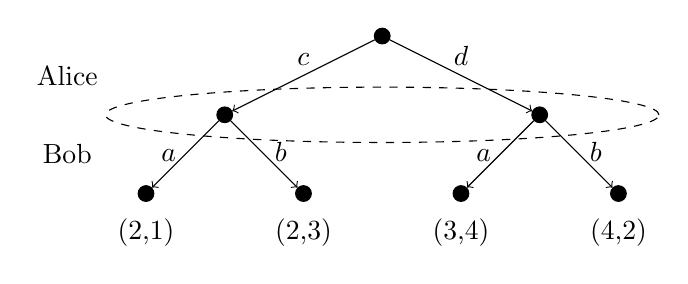
\begin{tikzpicture}
    \node[draw,circle,inner sep=.2em,fill=black] (n1) at (0,0) {};
    \node[draw,circle,inner sep=.2em,fill=black] (n2) at (-2,-1) {};
    \node[draw,circle,inner sep=.2em,fill=black] (n3) at (2,-1) {};
    \node[draw,circle,inner sep=.2em,fill=black] (n4) at (-3,-2) {};
    \node[draw,circle,inner sep=.2em,fill=black] (n5) at (-1,-2) {};
    \node[draw,circle,inner sep=.2em,fill=black] (n6) at (1,-2) {};
    \node[draw,circle,inner sep=.2em,fill=black] (n7) at (3,-2) {};
    \draw [->] (n1) -- node[above] {$c$} (n2);
    \draw [->] (n1) -- node[above] {$d$} (n3);
    \draw [->] (n2) -- node[above, near end] {$a$} (n4);
    \draw [->] (n2) -- node[above, near end] {$b$} (n5);
    \draw [->] (n3) -- node[above, near end] {$a$} (n6);
    \draw [->] (n3) -- node[above, near end] {$b$} (n7);
    \draw (-4,-.5) node {Alice}
          (-4,-1.5) node {Bob}
          (-3,-2.5) node {(2,1)}
          (-1,-2.5) node {(2,3)}
          (1,-2.5) node {(3,4)}
          (3,-2.5) node {(4,2)};
    \draw [style=dashed] (0,-1) ellipse (10em and 1em);

  \end{tikzpicture}
\end{center}
  \end{minipage}
  \caption{Game in extended form that corresponds to the normal form
  game from Figure~\ref{fig:stanform}.}
  \label{fig:ext-form}
\end{SCfigure}


Figure~\ref{fig:ext-form} shows the extended form version of the
payoff matrix from figure~\ref{fig:stanform}. In it, the first number
inside the parentheses is the utility that Bob receives and the second
number is Alice's utility.  The dotted line groups together two states
which are invisible to Bob: it shows that Bob does not know the action
Alice took. If we eliminated the dotted line then in that new game
Alice takes an action, which Bob can see, and then Bob takes his
action.

\mc{Extended form games, without the dotted ellipses, are nearly
  identical those built by the minimax algorithm \cite[Chapter
  6]{russell03a}. }

In an extended game a player's strategy $s_i$ is no longer just an
action but can now be a series of actions if the player gets to take
more than one action in the tree, or if the player can have different
actions depending on which node in the tree it is in. That is, if a
player can see others' actions that come before him then his action
can vary. For example, in figure~\ref{fig:ext-form2} a rational Bob
would choose $b$ if Alice has chosen $c$ but would choose $a$ if Alice
has chosen $d$. As before, agent $i$'s utility from strategy $s$ is
given by $u_i(s)$ and corresponds to the values on the leaf node
reached when all players play $s$.


\begin{SCfigure}
  \begin{minipage}{1.0\linewidth}
\begin{center}
  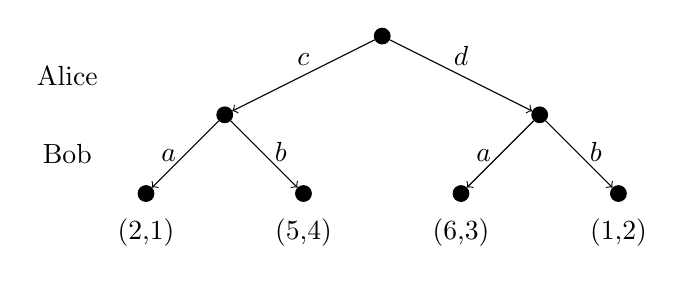
\begin{tikzpicture}
    \node[draw,circle,inner sep=.2em,fill=black] (n1) at (0,0) {};
    \node[draw,circle,inner sep=.2em,fill=black] (n2) at (-2,-1) {};
    \node[draw,circle,inner sep=.2em,fill=black] (n3) at (2,-1) {};
    \node[draw,circle,inner sep=.2em,fill=black] (n4) at (-3,-2) {};
    \node[draw,circle,inner sep=.2em,fill=black] (n5) at (-1,-2) {};
    \node[draw,circle,inner sep=.2em,fill=black] (n6) at (1,-2) {};
    \node[draw,circle,inner sep=.2em,fill=black] (n7) at (3,-2) {};
    \draw [->] (n1) -- node[above] {$c$} (n2);
    \draw [->] (n1) -- node[above] {$d$} (n3);
    \draw [->] (n2) -- node[above, near end] {$a$} (n4);
    \draw [->] (n2) -- node[above, near end] {$b$} (n5);
    \draw [->] (n3) -- node[above, near end] {$a$} (n6);
    \draw [->] (n3) -- node[above, near end] {$b$} (n7);
    \draw (-4,-.5) node {Alice}
          (-4,-1.5) node {Bob}
          (-3,-2.5) node {(2,1)}
          (-1,-2.5) node {(5,4)}
          (1,-2.5) node {(6,3)}
          (3,-2.5) node {(1,2)};
  \end{tikzpicture}
\end{center}
  \end{minipage}
  \caption{Game in extended form.}
  \label{fig:ext-form2}
\end{SCfigure}



\subsection{Solution Concepts}
\label{sec:solution-concepts}

We can apply the Nash equilibrium idea from normal form games to
extended games. Namely, we say that an extended game has a Nash
equilibrium strategy $s^*$ if for all agents $i$ it is true that they
can't gain any more utility by playing a strategy different from
$s^*_i$ given that everyone else is playing $s^*_{-i}$. For example,
for the game in figure~\ref{fig:ext-form2} the Nash equilibrium is
$(c,b)$---Alice plays $c$ and Bob plays $b$. While this strategy is in
equilibrium notice how, if there was some problem or noise in the
system and Alice ends up playing $d$ then Bob's strategy of playing
$b$ is no longer his best response. That is, the basic Nash
equilibrium solution might not be stable under noisy conditions.

A stronger solution concept is the \td{subgame perfect equilibrium}
strategy $s^*$ which is defined as one where for all agents $i$ and
all subgames it is true that $i$ can't gain any more utility by
playing a strategy different from $s^*_i$. We define a subgame to be
any subtree of the extended game. That is, a subgame perfect
equilibrium gives all the agents their best response strategies for
every node in the tree. For example, the subgame perfect equilibrium
for figure~\ref{fig:ext-form2} is for Alice to play $c$ and Bob to
play $b$ if Alice plays $c$ and $a$ if Alice plays $d$.

\medskip

Extended form games are a useful way to represent more complex
multiagent interactions. Notice, however, that they are a special case
of a multiagent Markov decision process. Most researchers have opted
to use the more complete Markov model over the simpler extended form
game for modeling multiagent systems.

These solution concepts provide us with solutions to shoot for when
building multiagent systems, even when these solutions are impossible
to find. For example, say you want to build a team of robot soccer
players. Each robot will have a specific behavior that depends on its
current perception of the world and its internal state. Each robot can
also be assumed to receive a payoff whenever it, or someone in its
team, scores a goal. If you consider the set of all possible agent
behaviors for all agents in the team as the set of actions in a game
then we can talk about the players being at a Nash equilibrium, or
about the players in one team being in the Pareto optimum given the
other team's behaviors. Of course, such equilibria are impossible to
calculate but they do give us a precise goal, of the intellectual
kind, to shoot for. Also, as many researchers have done, we can try to
break up that immense problem into smaller problems for which the
agents can find equilibrium strategies.

\section{Finding a Solution}

There is an extensive literature on centralized algorithms for finding
the various equilibrium strategies for a given game they are, however,
generally considered to be outside the purview of multiagent research.
Generally, the algorithms involve a complete search using heuristics
for pruning.  The \td{Gambit} software program \cite{mckelvey06a} is
an open source implementation of several of these algorithms.

However, note that some of these solutions can be found by more
multiagent-friendly distributed algorithms. In
chapter~\ref{cha:learn-mult-syst} we show multiagent learning
algorithms which allow learning agents to converge to Nash and other
equilibria.


\begin{exercises}
\item Prove that a social welfare solution must be Pareto optimal.

\item Show a 2-person standard form game with 3 actions for each
  player in which iterated dominance leads to a unique equilibrium
  strategy.
\item Assume a 2-person standard form game with $x$ actions for each
  player.
  \begin{enumerate}
  \item What is the maximum number of Pareto optimal pure strategies
    that such a game could have?
  \item Assuming that all payoff values are different, what is the
    maximum number of Pareto optimal pure strategies that such a game
    could have?
  \end{enumerate}

\item Find the pure Nash equilibria, and the Pareto optimal solutions
  of the following game:

    \begin{center}
      \renewcommand\arraystretch{1.5}
      \begin{tabular}{cc|c|c|c|}
        &    &\multicolumn{3}{c}{Alice} \\ 
        &      &$d$&$e$&$f$ \\ \cline{1-5}
        \multirow{3}{2em}{Bob}
        & $a$  &1,2 &2,3 &2,3 \\ \cline{2-5}
        & $b$  &4,5 &6,7 &3,4 \\ \cline{2-5}
        & $c$  &5,4 &6,5 &5,6 \\ \cline{2-5}
      \end{tabular}
    \end{center}


\item The battle of the sexes game, seen in figure~\ref{fig:battlesex}, is a
  classic coordination game in which the players must somehow
  coordinate to agree upon one of the Nash equilibria. These
  problems are solved by populations who adopt a \idx{social law}
  after some trial and error adaptation phase. For example, in the US
  people drive on the right side of the rode while in England they
  drive on the left. Both solutions are equally valid.

  \netlogo{coordination} Implement a NetLogo program where each patch
  repeatedly engages in a battle of the sexes game with one of its
  neighbors, chosen at random. Then try to come up with some simple
  adaptation strategy which the agents could use so that the
  population will quickly converge to an equilibrium.

  Simple adaptation strategies for solving this problem exist
  \cite{shoham97a}, as well as for more complex neighborhood
  definitions \cite{delgado02a}.

\item Lets say that in a repeated version of the game of chicken,
  figure~\ref{chicken}, Alice and Bob decided to converge to the
  strategy (Swerve, Swerve). Since this strategy satisfies the
  maxmin criteria (check this) the Folk theorem tells us that is will
  be stable since both players could play an iterated strategy that
  penalizes the other so that any gains from defection are erased
  after some rounds. Write the short algorithm which describes the
  player's iterated strategy for this situation, that is, the iterated
  strategy they must use to guarantee that (Swerve, Swerve) is the
  equilibrium strategy on every step of the iterated game.

\item A generalization of the Tit-for-Tat strategy is to, instead of
  simply doing exactly what the other agent did last time, make a
  stochastic decision based on the other agent's action. That is, if
  the other agent defected last time then you will be very likely,
  with a given probability, to defect and vice versa. Write a NetLogo
  program where you add these type of agents to a tournament similar
  to Axelrod's. Which strategy triumphs in the end?

  \netlogo{packages} This general strategy is known as
  \idx{reciprocity} and often occurs in human interaction: you are
  more likely, but not entirely sure, to be nice to those that were
  nice to you in the past. Simulations of populations with various
  numbers of reciprocating agents have shown that populations of
  reciprocating agents tend to do better as a whole (since they help
  each other) but can be exploited by selfish agents. This
  exploitation can be curbed by having the reciprocating agents share
  their opinions of other \cite{sen02b}.

\end{exercises}


\chapter{Characteristic Form Games and Coalition Formation}
\label{sec:games-char-form}

There is another type of game studied in game theory: the
\td{characteristic form} game or \td{coalition} game
\cite{osborne99a}. In these games the agents decide how to form
coalitions among themselves and each coalition receives some utility.
For example, a group of people, each with different skills, all want
to start new companies.  The problem they face is deciding how to
divide themselves into subgroups such that each subgroup has the
needed set of skills to succeed in the marketplace.  Similarly, a
group of agents with different skills must decide how to divide itself
into subgroups so as handle as many tasks as possible in the most
efficient manner. Because the agents must cooperate with each other in
order to form coalitions and an agent cannot unilaterally decide that
it will form a coalition with a second agent, these games are known as
\td{cooperative games}. Multiagent researchers have also extended the
basic characteristic form into to the more general coalition
formation, which we also present in this chapter.

It is interesting to note that most game theory textbooks focus
exclusively on non-cooperative games as these have found many
applications in Economics and Business and have been the focus of most
of the research. However, when building multiagent systems we find
that cooperative games are much more useful since they clearly and
immediately model the problem of which agents should perform which
tasks.

\section{Characteristic Form Games}
\label{sec:char-form-games}

Formally, a game in characteristic form includes a set $A =
\{1,\ldots, |A|\}$ of agents. The agents are assumed to deliberate and
the final result of the deliberation is an \td{outcome} $\vu =
(u_1,\ldots,u_{|A|}) \in \Re^{|A|}$ which is just a vector of
utilities, one for each agent. There is also a rule $V(\cdot)$ that
maps every coalition $S \subset A$ to a utility possibility set, that
is $V(S) \subset \Re^{|S|}$. Notice that $V(S)$ returns a set of
utility vectors, not a single utility vector. As such, $V(\cdot)$
provides us the set of payoffs that players in $S$ can achieve it they
form a coalition. For example, for the players $\{1,2,3\}$ we might
have that $V(\{1,2\}) = \{(5,4),(3,6)\}$ meaning that if agents 1 and
2 formed a coalition they could either get 5 for agent 1 and 4 for
agent 2, or they could get 3 for agent 1 and 6 for agent 2. The
function $V$ must be defined for all subsets of $A$.

A special case of the characteristic form game--the one nearly all
multiagent research focuses on---is the \td{transferable utility} game
in characteristic form. This game assumes that the players can
exchange utilities among themselves as they see fit. For example, if
the utility payments are in the form of money then we only need to
specify the total amount of money the coalition will receive and
decide later how this money will be distributed among the agents in
the coalition.  More formally, we define a transferable utility game

\begin{definition}[Tranferable utility characteristic form game] These
  games consist of a set of agents $A = \{1,\ldots,A\}$ and a
  \emph{characteristic function} $v(S) \rightarrow \Re$ defined for
  every $S \subseteq A$.
\end{definition}

The \td{characteristic function} $v(S)$ is also sometimes simply
referred to as the \td{value function} for the coalitions.
Characteristic form games with transferable utility can represent many
multiagent scenarios. For example, they can represent a task
allocation problem where a set of tasks has to be performed by a set
of agents, subsets of whom can sometimes improve their performance by
joining together to perform a task. They can represent a sensor
network problems where the sensors must join together in subgroups to
further refine their readings or relay important information, or they
can represent workflow scheduling systems where agents must form
groups to handle incoming workflows.

\subsection{Solution Concepts}

As is often the case in game theory, there is no clear best solution
to all characteristic form games. Instead, various solutions concepts
have been proposed each one having its own advantages and
disadvantages.

Before defining the solution concepts, we must first notice that the
outcome as we have defined it allows for impossible utility values in
the transferable utility game. Specifically, there might not be a set
of coalitions such that, given $v$, the agents can all get their
utility as promised by \vu{}. In order to rectify this problem we
first specify that we are only interested in \td{feasible} outcomes,
that is, those that can be implemented given $v$.

\begin{definition}[Feasible]
  An outcome $\vu$ is \emph{feasible} if there exists a set of
  coalitions $T = S_1,\ldots,S_k$ where $\bigcup_{S \in T} S = A$
  such that $\sum_{S \in T} v(S) \geq \sum_{i \in A} \vu_i$.
\end{definition}

That is, an outcome $\vu$ is feasible if we can find a disjoint set of
coalitions whose values are as much as that in $\vu$, so we can payoff
$\vu$ with $v$. The set of disjoint coalitions $T$ defined above is
also often referred to as a \td{coalition structure}, also sometimes
represented with the symbol $CS$.

Notice that, if the characteristic function is super-additive then we
can check if an outcome \vu{} is feasible by simply ensuring that
\begin{equation}
  \label{eq:gt-7}
  \sum_{i \in A} \vu_i = v(A).
\end{equation}
We define a \td{super-additive} domain as one where, for all pairs of
disjoint coalitions $S,T \subset A$, we have that $v(S \cup T) \geq
v(S) + v(T)$. That is, there is nothing to be lost by merging into a
bigger coalition. Unfortunately, multiagent systems are rarely
supper-additive since agents have a habit of getting into each others'
way, so that a team is not always better than letting each agent work
on a task separately.

\begin{SCfigure}
  \begin{minipage}{1.0\linewidth}
  \begin{center}
    \begin{tikzpicture}
      \node (n1) at (0,1.5) {\snugbox{$(1)(2)(3)$\\$2 + 2 + 4 =8$}};
      \node (n2) at (-3,0) {\snugbox{$(1)(23)$\\$2 + 8 = 10$}};
      \node (n3) at (0,0) {\snugbox{$(2)(13)$\\$2 + 7 = 9$}};
      \node (n4) at (3,0) {\snugbox{$(3)(12)$\\$4 + 5 = 9$}};
      \node (n5) at (0,-1.5) {\snugbox{$(123)$\\$9$}};
      \node (v) at (-6,0){
        \begin{tabular}{cr} \toprule
          $S$ & $v(S)$ \\ \midrule
          $(1)$ & \emph{$2$} \\ 
          $(2)$ & \emph{$2$}\\ 
          $(3)$ & \emph{$4$}\\ 
          $(12)$& \emph{$5$}\\ 
          $(13)$& \emph{$7$}\\ 
          $(23)$& \emph{$8$}\\ 
          $(123)$& \emph{$9$}\\ \bottomrule
        \end{tabular}};
    \end{tikzpicture}
  \end{center}
  \end{minipage}
  \caption{Sample characteristic form game with transferable utility
    for three agents: 1, 2 and 3.  The table on the left shows the
    values of each coalition. On the right are the coalition
    structures. Below each one we calculate its value.}
  \label{fig:ex1}
\end{SCfigure}
The problem of finding feasible solutions can best be illustrated with
an example.  Figure~\ref{fig:ex1} shows a sample transferable utility
game for three agents along with the definition of the $v$ function
and all possible coalition formations. In this game the outcome $\vu =
\{5,5,5\}$ is not feasible since there is no way to divide the agents
into subsets such that they can all get their utility. If we tried the
coalition $(123)$ then we only have a value of 9 to distribute and we
need a total of 15. On the other hand, the outcome $\vu = \{2,4,3\}$,
is feasible because the coalition structures $(1)(23)$, $(2)(13)$, and
$(123)$ can satisfy it (but not the other ones). However, $\vu =
\{2,4,3\}$ does have a problem in that in it agent 3 is getting an
utility of 3 while we have that $v((3)) = 4$. That is, agent 3 could
defect any one of the three coalition structures we found, join the
coalition $(3)$, and get a higher utility than he currently has. This
outcome thus seems unstable.

\subsubsection{The Core}

%Add simplex graph to show outcomes in the core.

In general, we say that an outcome $\vu$ is stable if no subset of
agents gets paid more, as a whole, than what they get paid in $\vu$.
Stability is a nice property because it means that the agents do not
have an incentive to go off into their own coalition. Our first
solution concept, the \td{core}, refers to all the outcomes that are
stable.

\begin{definition}[Core]
  \label{def:core}
  An outcome $\vu$ is in the \emph{core} if
  \begin{enumerate}
  \item     \[\forall_{S \subset A}: \sum_{i \in S} \vu_i \geq v(S)\]
  \item it is feasible.
  \end{enumerate}
\end{definition}
The first condition in this definition tells us that the utility the
agents receive in outcome $\vu$ is bigger than those of any coalition,
for the agents in the coalition. In other words, that there is no
coalition $S$ whose $v(S)$ is bigger than the sum of payments the
agents in $S$ get under $\vu$. The second condition merely checks that
the total utility we are giving out is not more than what is coming in
via $v(\cdot)$.

\begin{SCfigure}
  \begin{minipage}{1.0\linewidth}
  \begin{center}
    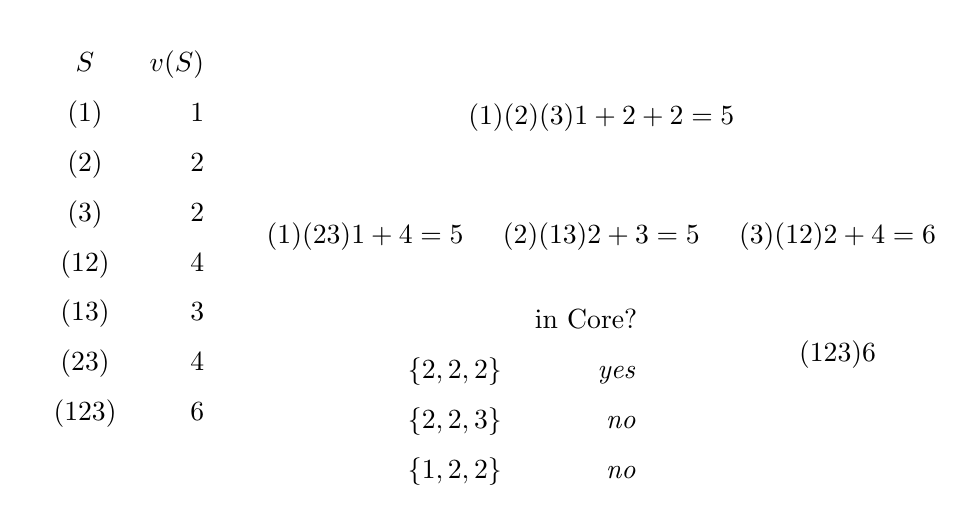
\begin{tikzpicture}
      \node (n1) at (0,1.5) {\snugbox{$(1)(2)(3)$\\$1 + 2 + 2 =5$}};
      \node (n2) at (-3,0) {\snugbox{$(1)(23)$\\$1 + 4 = 5$}};
      \node (n3) at (0,0) {\snugbox{$(2)(13)$\\$2 + 3 = 5$}};
      \node (n4) at (3,0) {\snugbox{$(3)(12)$\\$2 + 4 = 6$}};
      \node (n5) at (3,-1.5) {\snugbox{$(123)$\\$6$}};

      \node (v) at (-6,0){
        \begin{tabular}{cr} \toprule
          $S$ & $v(S)$ \\ \midrule
          $(1)$ & \emph{$1$} \\ 
          $(2)$ & \emph{$2$}\\ 
          $(3)$ & \emph{$2$}\\ 
          $(12)$& \emph{$4$}\\ 
          $(13)$& \emph{$3$}\\ 
          $(23)$& \emph{$4$}\\ 
          $(123)$& \emph{$6$}\\ \bottomrule
        \end{tabular}};

      \node (u) at (-1,-2){
        \begin{tabular}{cr} \toprule
          $\vu$ & in Core? \\ \midrule
          $\{2,2,2\}$ & \emph{yes} \\ 
          $\{2,2,3\}$ & \emph{no} \\ 
          $\{1,2,2\}$ & \emph{no} \\ \bottomrule
        \end{tabular}};
    \end{tikzpicture}
  \end{center}
  \end{minipage}
  \caption{Sample game showing some outcomes that are
    in the core and some that are not. The characteristic function
    $v$ is super-additive.}
  \label{fig:ex2}
\end{SCfigure}


\mpic{gametheory/shapley}{Lloyd F. Shapley}{1923}{}{Responsible for
  the core and Shapley value solution concepts.}  Figure~\ref{fig:ex2}
shows a new game with different payments and a list of outcomes some
of which are in the core and some which are not.  $\{2,2,2\}$ is in
the core because it is feasible and there is no subset of agents $S$
with a $v(S)$ that is bigger than what they could get in this outcome.
$\{2,2,3\}$ is not in the core because it is not feasible. This
outcome adds up to 7 and there is no coalition structure that adds up
to 7. Note that, since the $v$ is super-additive, all we need to check
is the grand coalition. Finally, $\{1,2,2\}$ is not in the core
because agents 1 and 2 are getting a total of 3 while if they formed
the coalition $(12)$ they would get a utility of 4.

We like the core because we know that any solution that is in the core
cannot be improved by having any of the $2^A$ subsets of agents form a
coalition of higher value than they are getting now. It is a very
stable solution. Unfortunately, there are many games with empty cores.
Figure~\ref{fig:emptycore} shows one such example. Try to find an
outcome in the core for this example. You will see that every outcome
is blocked by some other outcome.

\begin{SCfigure}
  \begin{minipage}{1.0\linewidth}
  \centering
  \begin{tabular}{cr} \toprule
    $S$ & $v(S)$ \\ \midrule
    $(1)$ & \emph{$0$} \\ 
    $(2)$ & \emph{$0$}\\ 
    $(3)$ & \emph{$0$}\\ 
    $(12)$& \emph{$10$}\\
    $(13)$& \emph{$10$}\\
    $(23)$& \emph{$10$}\\
    $(123)$& \emph{$10$}\\ \bottomrule
  \end{tabular}
  \end{minipage}
  \caption{Set of payments for a game with an empty core}
  \label{fig:emptycore}
\end{SCfigure}

% \cite{sandholm97b} defines a bounded rational core where there is a
% cost associated with calculating $v(s)$.

Another problem with the core solutions is that when it is not empty
then there are often many outcomes in the core. For example, in
figure~\ref{fig:ex2} any outcome $\vu = \{x,y,z\}$ where $x + y + z
\leq 6$ and $x + y \geq 4$ and $x + z \geq 3$ and $y + z \geq 4$ is in
the core. Thus, we still have a coordination or negotiation problem
where we must choose between these coalitions. Finally, there is the
fact that the outcome does not tell us which coalitions are
formed. For example, if we choose the outcome $\vu = \{2,2,2\}$ then
we must still also choose a coalition structure as there are two
which would work: $(123)$ and $(12)(3)$.


\subsubsection{The Shapley Value}

While the core gives us one possible solution, it suffers from the
fact that many games don't have any solutions in the core and from its
lack of guidance in fairly distributing the payments from a coalition
to its members. The Shapley value solves these problems by giving us
one specific set of payments for coalition members, which are deemed
fair.

\begin{SCfigure}
  \begin{minipage}{1.0\linewidth}
  \centering
  \begin{tabular}{cr} \toprule
    $S$ & $v(S)$ \\ \midrule
    $()$ & \emph{$0$} \\ 
    $(1)$ & \emph{$1$} \\
    $(2)$ & \emph{$3$}\\ 
    $(12)$& \emph{$6$}\\ \bottomrule
  \end{tabular}
  \end{minipage}
  \caption{Example game. If the agents form coalition $(12)$ then how
    much utility should each one get?}
  \label{fig:ex3}
\end{SCfigure}


The problem with identifying fairness in characteristic form games is
best illustrated by an example. Figure~\ref{fig:ex3} shows a game for
two players. Clearly, we should choose the coalition $(12)$ as it has
the highest value. Now we must decide how much each agent should get.
The simplest solution is to divide the total of 6 evenly amongst the
coalition members, so that each agent gets 3. This seems unfair to
agent 2 because agent 2 could have gotten 3 by simply staying on its
own coalition $(2)$. It seems like the fair thing to do is to give
each agent a payment that is proportional to the value it contributes
to the coalition, that is, the amount that value increases by having
the agent in the coalition. But, how do we extend this idea to cases
with more than 2 agents?

Shapley was able to extend this idea by realizing that each agent
should get a payment that corresponds to its marginal contribution to
the final value. An agent's marginal contribution to a coalition is
the difference between the value before the agent joins the coalition
and after he joined. For example, if before you join Initech their
annual profits are \$10M but after you are there for a year they
increase to \$11M then you can claim that your marginal contribution
is to Initech is \$1M assuming, of course, that everything else stays
the same during that year.

The one remaining problem is that there are many different orderings
in which $n$ agents could have joined the coalition, namely, there are
$n!$ orderings of $n$ elements. The \td{Shapley value} simply averages
over all possible orderings. That is, the Shapley value gives each
agent a utility proportional to its average marginal contribution to
every possible coalition, in every possible order it could have been
formed. More formally, we define the Shapley value as:

\begin{definition}[Shapley Value]
  Let $B(\pi,i)$ be the set of agents in the agent ordering $\pi$
  which appear before agent $i$. The \emph{Shapley value} for agent $i$
  given $A$ agents is given by
  \[ \phi(A,i) = \frac{1}{A!} \sum_{\pi \in \Pi_A} v(B(\pi,i) \cup i) -
  v(B(\pi,i)), \]
  where $\Pi_A$ is the set of all possible orderings of the set
  $A$. Another way to express the same formula is 
  \[ \phi(A,i) = \sum_{S\subseteq A} \frac{(|A|-|S|)! \,(|S| - i)!}{|A|!}
  [v(S) - v(S - \{i\})].\]
\end{definition}

Notice that the Shapley values are calculated for a particular
coalition $A$ in the definition above. They are not meant as a way of
determining which is the best coalition structure. They can only be
used to distribute the payments of a coalition once it is formed.

Lets calculate the Shapley values for the game in figure~\ref{fig:ex3}
and the grand coalition $(12)$. Since there are only two agents it
means that there are only two possible orderings: $(12)$ and $(21)$.
As such we have that

\begin{eqnarray*}
  \phi(\{1,2\}, 1) &=&\frac{1}{2}\cdot \left( v(1) - v() + v(21) -
    v(2)\right)\\
  &=&\frac{1}{2}\cdot( 1 - 0 + 6 - 3) = 2 \\
  \phi(\{1,2\}, 2) &=&\frac{1}{2}\cdot \left( v(12) - v(1) + v(2) -
    v()\right)\\
  &=&\frac{1}{2}\cdot( 6 - 1 + 3 - 0) = 4
\end{eqnarray*}
A somewhat surprising and extremely useful characteristic of the
Shapley value is that it is always feasible. In our example the
payments of 4 and 2 add up to 6 which is the same value we get in the
grand coalition $(12)$.  Another nice feature of the Shapley value is
that it always exists and is unique. Thus, we do not have to worry
about coordination mechanism to choose among different payments. A
final interesting result is that the Shapley value might not be in the
core, even for cases where the core exists. This is a potential
problem as it means that the resulting payments might not be stable
and some agents might choose to leave the coalition in order to
receive a higher payment on a different coalition.

%mas-colell glove market, p681

Unfortunately, while the Shapley value has some very attractive
theoretical properties, it does have some serious drawbacks when we
try to use it for building multiagent systems. The biggest problem is
computational. The Shapley value requires us to calculate at least
$2^{|A|}$ orderings, this is only possible for very small sets $A$. It
also requires that we know the value of $v$ for every single subset
$S$.  In many real-world applications the calculation of $v$ is
complex. For example, it might require simulating how a particular
coalition of agents would work together. These complex calculations
could dramatically increase the total time. Finally, the Shapley value
does not give us the actual coalition structure. Thus, it only solves
the second part of the coalition formation problem. We must still
determine which coalition the agents will form and how they will do
it.

\subsubsection{The Nucleolus}
\label{sec:nucleolus}

Since the core is often empty, researchers started looking for ways of
relaxing it and find a new solution concept that would exist for every
game. The problem with the core is that it says that there is no
subset of agents that could get paid more than what they are currently
getting paid in $\vu$, because then they would be tempted to
defect and form a new coalition. If it is impossible to find such an
$\vu$ then the next best thing would be to find the
$\vu$ that minimizes the total temptation felt by the agents.
That is what the \td{nucleolus} aims to do.

We start by clarifying what we mean by temptation. Specifically, a
coalition $S$ is more tempting the higher its value is over what the
agents get in $\vu$. This is known as the \td{excess}.
\begin{definition}[excess]
  The \emph{excess} of coalition $S$ given outcome \vu{} is
  given by 
  \[e(S,\vu) = v(S) - \vu(S), \]
  where 
  \[\vu(S) = \sum_{i\in S} \vu_i.\]
\end{definition}

That is, a coalition $S$ has a positive excess, given \vu{}, if the
agents in $S$ can get more from $v(S)$ than they can from \vu{}. The
more they can get from $S$ the higher the excess. Note that, by
definition, if an outcome \vu{} is in the core then all coalitions
have a excess that is less than or equal to 0 with respect to that
outcome.  But, since we are now concerned with outcomes that are not
in the core we will instead look for those with minimal excess. Since
excess is defined for all possible subsets $S$ we first need a way to
compare the excesses of two outcomes. We do this by putting them in a
sorted list and comparing the list. The one with the higher excess
first is declared more excessive. More formally, for each \vu{} we
find its excess for all subsets $S$ and order these in a list; the
higher excesses come first, as such
\begin{equation}
  \label{eq:gt-8}
  \theta(\vu) = \langle e(S_1^{\vu},\vu), e(S_2^{\vu},\vu),\ldots
  ,e(S_{2^{|A|}}^{\vu},\vu) \rangle,
\end{equation}
where $e(S_i^{\vu}, \vu) \geq e(S_j^{\vu}, \vu)$ for all $i < j$.  We
then define a lexicographical ordering $\succ$ over these lists where
$\theta(\vu) \succ \theta(\vv)$ is true when there is some number $q
\in 1\ldots 2^{|A|}$ such for all $p < q$ we have that
$e(S_p^{\vu},\vu) = e(S_p^{\vv},\vv)$ and $e(S_q^{\vu},\vu) >
e(S_q^{\vv},\vv)$ where the $S_i$ have been sorted as per $\theta$.
That is, if $\theta(\vu) \succ \theta(\vv)$ then that means that when
we sort their excesses for all subsets their first, and greatest,
excesses are all the same and on the first set for which they have a
discrepancy \vu{} has the highest excess. For example, if we had the
lists $\{(2,2,2), (2,1,0), (3,2,2), (2,1,1)\}$ they would be ordered
as $\{(3,2,2), (2,2,2), (2,1,1), (2,1,0)\}$.

We can now define the \td{nucleolus} as the \vu{} which is not
lexicographically bigger than anyone else.
\begin{definition}[nucleolus]
  The \emph{nucleolus} is the set
  \[ \{\vu{} \,|\, \theta(\vu) \not{\succ} \theta(\vv) \text{ for all }
  \vv \text{, given that } \vu \text{ and } \vv \text{ are feasible.}\}\]
  
\end{definition}
In other words, the outcomes in the nucleolus are those where the
excesses for all possible sets are lexicographically not greater than
those of any other outcome. A nice feature of the nucleolus is that it
is always unique for each coalition structure. That is, given a
coalition structure there is only one nucleolus.

The nucleolus captures, to some degree, the idea of an outcome that
minimizes the temptation the agents face. However, notice that the
lexicographic order it defines only cares about the first coalition
that has a higher excess, it does not care about the ones after that.
This could lead to a situation where the sum of the excesses from the
nucleolus is actually larger than that of some other outcome. For
example, $(5.0,0,0)$ comes before $(4,3,3,3)$. As such, the nucleolus
does not seem to minimize the sum of temptations.

\subsubsection{Equal Excess}
\label{sec:equal-excess}

Another technique for calculating the agents' payoff, besides the
Shapley value, is called \td{equal excess}. It is an iterative
algorithm where we adjust the payments that the agents expected they
will receive from each coalition that includes them. At each time step
$t$ we let $E^t(i,S)$ be agent $i$'s expected payoff for each
coalition $S$ which includes him. Initially these are set to 0. We
thus let
\begin{equation}
  \label{eq:gt-9}
  A^t(i,S) = \max _{T \neq S} E^t(i,T)  
\end{equation}
be agent $i$'s expected payment from not choosing $S$ and instead
choosing the best alternative coalition. Then, at each time step we
update the players' expected payments using
\begin{equation}
  \label{eq:gt-10}
  E^{t+1}(i,S) = A^t(i,S) + \frac{v(S) - \sum_{j\in S} A^t(j,S)}{|S|}.
\end{equation}

For example, for the value function given in figure~\ref{fig:ex3} we
start with $E^0(1,*)=E^0(2,*)=0$. Then, at time 1 agent 1 can update
$E^1(1,(1)) = 1$ and $E^1(1,(12)) = 3$ and then $A^1(1,(1)) = 3$ and
$A^1(1,(12)) = 1$, while agent 2 updates $E^1(2,(2)) = 3$ and
$E^1(2,(12)) = 3$ and then $A^1(1,(1)) = 3$ and $A^1(1,(12)) = 3$.

It has been shown that this basic algorithm does not always converge
to a fixed point, however, variations of it have been proposed which
do converge, such as \acro{pact} \cite{goradia07b}. In \acro{pact} the
agents calculate their own $E$ values and exchange them with others
under the assumption that agents will not lie about these values. The
algorithm ensures that the process will stop and a solution will be
found.

Notice that equal excess is a procedural solution to the problem so we
do not know which specific outcome the agents will converge to, other
than to say that they will converge to the outcome that is found when
we use equal excess.


% Note that, since the equal excess procedure requires us to know the
% $A$ values of all agents it is a centralized procedure. However, it
% does not seem impossible that we could parallelize this procedure by
% having the agents exchange $A$ values. \mc{Exercise: Give an example
%   when an agent would want to lie.} Unfortunately, in such a scenario
% it would not be in the agents' best interest to tell the truth about
% its current $A$.

% Yet another equilibrium concept is the kernel (Osborne and
% Rubenstein) which is always non-empty.

\subsection{Finding the Optimal Coalition Structure}

As multiagent system designers we often simply want to find the
outcome that maximizes the sum of values. That is, we want to find the
\td{utilitarian} solution. When the characteristic function is
super-additive then the grand coalition will have the highest value
and thus finding the utilitarian solution is trivial. However, if the
characteristic is not super-additive---as is often the case in
multiagent systems---then we will want an algorithm for finding it.
Notice that under this formulation we are no longer interested in the
specific outcome (that is, individual payments to agents) we are now
only interested in finding best coalition structure, ignoring the
problem of dividing up the value of each coalition among its
participants.

\subsubsection{Centralized Algorithm}
\begin{SCfigure}
  \begin{minipage}{1.0\linewidth}
  \begin{center}
    \begin{tikzpicture}[style=dstyle]
%      \useasboundingbox (-5,-1.5) rectangle (5,2);
      \node at (0,2) {$(1)(2)(3)(4)$};

      \node at (-5,1) {$(12)(3)(4)$};
      \node at (-3,1) {$(13)(2)(4)$};
      \node at (-1,1) {$(14)(2)(3)$};
      \node at (1,1) {$(23)(1)(4)$};
      \node at (3,1) {$(24)(1)(3)$};
      \node at (5,1) {$(34)(1)(2)$};

      \node at (-5,0) {$(1)(234)$};
      \node at (-3.33,0) {$(2)(134)$};
      \node (n1) at (-1.67,0) {$(3)(124)$};
      \node at (0,0) {$(4)(123)$};
      \node at (1.67,0) {$(12)(34)$};
      \node at (3.33,0) {$(14)(23)$};
      \node at (5,0) {$(13)(24)$};

      \node (n2) at (0,-1) {$(1234)$};
%      \node[color=gray] (t) at (-4,-2) {All possible coalitions};
%      \draw[color=gray,->] (t) -- (n1);
%      \draw[color=gray,->] (t) -- (n2);
    \end{tikzpicture}
  \end{center}
  \end{minipage}
  \caption{Coalition structure formation possibilities for four
    agents, organized by the number of coalitions.}
  \label{fig:brute}
\end{SCfigure}

One proposed approach is to a perform a complete search of the
complete set of possible coalition structures, but in a specified
order. Figure~\ref{fig:brute} shows all the possible coalition
structures for four agents. Notice that the bottom two rows contain
all possible coalitions. This means that after searching those two
rows we have seen all possible coalitions. If we let $S^*$ be the
value of the highest valued coalition (\emph{not} coalition structure)
found after searching those two rows then we know that the best
coalition structure cannot be more than $A\cdot S^*$. As such, after
searching the bottom two levels we can say that the optimal solution
is no more than $A$ times better than the best solution we have found
thus far.

\begin{SCfigure}
  \begin{minipage}{1.0\linewidth}
  \begin{center}
    \begin{tabular}{cc}\toprule
      Level&Bound \\ \midrule
      $A$  &$A/2$ \\ 
      $A-1$&$A/2$ \\ 
      $A-2$&$A/3$ \\ 
      $A-3$&$A/3$ \\ 
      $A-4$&$A/4$ \\ 
      $A-5$&$A/4$ \\ 
      :    &:  \\ 
      2    &$A$ \\ 
      1    &none  \\ \bottomrule
    \end{tabular} 
  \end{center}
  \end{minipage}
  \caption{Bounds on optimality after searching various levels.}
  \label{fig:bounds}
\end{SCfigure}

Figure~\ref{fig:bounds} shows the bounds that can be calculated after
examining each of the levels in the graph. One simple algorithm
consists of first searching the bottom two levels then continue
searching down from the top level \cite{sandholm99b}. In this way, the
bound from optimal is reduced as indicated in the figure.  Note that
searching the levels in some other order will not guarantee these
bounds. Notice also that the number of coalition structures in the
second level is given by its \td{Stirling} number
\begin{equation}
  \label{eq:stirling}
\text{Stirling}(A,2) = \frac{1}{2} \sum_{i=0}^{1} (-1)^i
\binom{2}{i}(2-i)^A = 2^{A-1} - 1.  
\end{equation}
So it takes exponential time just to search the second level. In
general, the number of coalition structures for all levels is equal to
the Stirling number for that level.

There also exists an algorithm for finding the optimal coalition
structure which has slightly better bounds than the ones we just
presented, but running time remains exponential and unusable for large
number of agents \cite{dang04a}.


\subsubsection{Distributed Algorithm}

While the previous algorithm found the optical coalition structure, it
did so at the expense of a lot of computation and in a centralized
manner. We now look at one possible way of finding a good, but
possibly not optimal, coalition structure in a decentralized manner.

\begin{SCfigure}
  \begin{minipage}{1.0\linewidth}
  \begin{codebox}
    \Procname{$\proc{Find-Coalition}(i)$}
    \li $L_i \gets$ set of all coalitions that include $i$. 
    \li $S_i^* \gets \arg \max_{S \in L_i} v_i(S)$
%    \li $w_i^* \gets v_i(S_i^*)$
    \li Broadcast $S_i^*$ and wait for all other broadcasts, put these
    into $S^*$ set.
    \li $S_{max} \gets \arg \max _{s \in S^*} v_i(s)$ 
    \li \If $i \in S_{\max}$
    \li \Then join $S_{\max}$
    \li \Return
    \End
    \li \For $j \in S_{\max}$
        \li \Do Delete all coalitions in $L_i$ that contain $j$
        \End
    \li \If $L_i$ is not empty 
    \li \Then goto 2
    \End
    \li \Return
  \end{codebox}
  \end{minipage}
  \caption{Distributed algorithm for coalition formation. Each agent
    $i$ must execute this function. We let $v_i(S) =
    \frac{v(S)}{|S|}$}
  \label{fig:dist}
\end{SCfigure}

\netlogo{find-coalition}Figure~\ref{fig:dist} shows a distributed
algorithm for coalition formation \cite{shehory98a}. The agents order
all their possible coalitions based on how much each will get in that
coalition, where each agent $i$ gets $v_i(S) = v(S)/|S|$ if it joins
coalition $S$. The agents then broadcast the name of their best
coalition. The coalition with maximal $v(S)/|S|$ is chosen by the
agents in $S$ who join the coalition and drop out of the algorithm.
The remaining agents take note of the missing agents by eliminating
from consideration all coalitions that include them. The process is
then repeated again with the new set of coalitions.

This is a classic example of a greedy or hill-climbing algorithm. As
such, we know that it might get stuck on a local optima, which might
or might not be the global optimum. Still, the algorithm should
execute very fast as there are at most $A$ steps and each step
involves having each agent examine all the possible coalitions that it
can be participate in.

A slight modification of the algorithm would be to, instead of
broadcasting at each time step we could let the agents meet randomly
and form a coalition if $v_i(s)$ is maximal for all agents in $s$.
Imagine the agents moving around in a space and forming sets whenever
a group of them happen to be close to each other, then forming a
coalition only if that set has a maximal value. This process is
effectively the same as broadcasting except that it eliminates the
need to broadcast at the expense of taking a longer time to converge
\cite{sarne07a}.


\subsubsection{Reduction to Constraint Optimization}
\label{sec:reduct-constr-optim}

We note that the problem of finding the optimal coalition structure
can be reduced to a constraint optimization problem. The basic idea is
that for $n$ agents there will be at most $n$ coalitions as, at worst,
each agent will stay in the individual coalition. Thus, we can imagine
the problem as consisting of $n$ agents each one deciding which of $n$
rooms to go into. The agents are the variables and the rooms are the
domains. The agents in a room form a coalition and empty rooms are
ignored. We set a constraint for each room equal to $- v(s)$ where $s$
is the set of agents that choose that room, or 0 if no agents choose
it.  We then have a constraint optimization problem where we are
trying to the set of values which minimizes the sum of the constraint
violations, thus maximizing the sum of the valuations.

Note that this is a degenerate case of the constraint optimization
problem in that all the $n$ constraints are over all agents. Most
constraint problems exhibit some degree of locality in that
constraints are only over a small subset of the variables. Having all
constraints be over all variables makes this problem harder than
average. Thus this reduction is likely to be only of theoretical
interest.


%\cite{shehory98a} seems to claim that the solution $CS$ found by this
%algorithm is bound by
%\[\frac{v(CS^*)}{v(CS)} \leq \sum_{i=1}^A \frac{1}{i}\] 
%but, I believe the following example contradicts that claim.

%\begin{SCtable}
%  \begin{minipage}{1.0\linewidth}
%    \begin{center}
%    \begin{tabular}{cc}\toprule
%      Coalition &$v(S)$ \\ \midrule
%      (1,2)  	&$2 x - \epsilon$\\ 
%      (1)	&$0$ \\ 
%      (2)	&$x$ \\ \bottomrule
%    \end{tabular}
%  \end{center}
%  \end{minipage}
%  \caption{Counterexample to bound claims.}
%  \label{tab:counter}
%\end{SCtable}
%Let $a = 2$ and the coalitions have the values as shown in
%Table~\ref{tab:counter}. For this case they predict that

%\[\frac{v(CS^*)}{v(CS)} \leq \frac{3}{2} \]

%but the algorithm would find $CS = (2)(1)$ which has $v(CS)
%= x$, while $v(CS) = 2x - \epsilon$ so 

%\[\frac{v(CS^*)}{v(CS)} = \frac{2x - \epsilon}{x} \leq \frac{3}{2} \]

%which, for small $\epsilon$ means that

%\[2 \leq \frac{3}{2}.\]

%I don't believe that we can place a theoretical bound on the quality
%of the solutions found by the \proc{Find-Coalition} algorithm for
%the general case. Perhaps under certain constrained situations, for
%example, if we limit the characteristic function. Other probabilistic
%bounds could be found via experimentation.


\section{Coalition Formation}
\label{sec:coalition-formation}

The \td{coalition formation} problem, as studied in multiagent
systems, extends the basic characteristic form game in an effort to
make it a better match for real world problems. A coalition formation
problem consists of three steps.
\begin{enumerate}
\item Agents generate values for the $v(\cdot)$ function.
\item Agents solve the characteristic form game by finding a suitable
  set of coalitions.
\item Agents distribute the payments from these coalitions to
  themselves in a suitable manner.
\end{enumerate}

Steps 2 and 3 can be thought of as part of the traditional
characteristic form game. The coalition formation definition simply
chooses to split the problem of finding a suitable outcome \vu{} into
two parts: finding the coalitions and then dividing the payments. The
split mirrors the requirements of many application domains. Step 1 is
completely new. It is there because in many domains it is
computationally expensive to determine the value of $v(S)$ for a given
$S$. For example, if the agents are trying to form groups that solve
particular tasks then calculating $v(S)$ requires them to determine
out how well they can perform the task as a group, which requires
considering how all their different skills can be brought to bear and,
in some common scenarios, requires the development of a full plan---an
exponential problem. The approaches at solving step 1 are thus
generally dependent on the domain and do not generalize well.




%In their abstract they say how it is ``up to $10^{379}$ times faster''
%than the other algorithm but that is just silly for they are talking
%about the case with 1000 agents where their algorithm searches about
%$10^{1100}$ coalition structures and the other algorithm searches
%about $10^{1500}$. Since the number of nanoseconds since the Big bang
%is smaller than $10^{100}$, their claim, while true, seems
%ridiculously out of place.
\begin{exercises}

\item Give an example problem in which agents using equal excess and
  reporting their own $E$ values will want to lie about their own $E$
  values.

\item Find the set of core solutions and the Shapley value of the
  grand coalition for the following game:
  \begin{tabular}{cr} \toprule
          $S$ & $v(S)$ \\ \midrule
          $(1)$ & \emph{$1$} \\ 
          $(2)$ & \emph{$2$}\\ 
          $(3)$ & \emph{$3$}\\ 
          $(12)$& \emph{$5$}\\ 
          $(13)$& \emph{$4$}\\ 
          $(23)$& \emph{$5$}\\ 
          $(123)$& \emph{$5$}\\ \bottomrule
        \end{tabular}


\item Say you have robots which live in a 2-dimensional grid and each
  one has a strength given by a number in the set $\{1,2,3,4,5\}$.
  There are boxes in this world, each one of which must be moved to a
  specified destination. The speed with which a set of robots $S$ can
  move a box is given by $1 - 1/\sum_{i \in S} i.\text{strength}$.
  \begin{itemize}
  \item Formulate this problem as a characteristic form game and
    provide a $v(S)$ definition.
  \item Find a good algorithm for calculating the optimal coalition
    structure.
  \end{itemize}

\item Modify the \proc{find-coalition} algorithm from
  figure~\ref{fig:dist} so that instead of the agents broadcasting
  their values they move around randomly in a two-dimensional space.
  After each time step the set of agents in a tile checks if they form
  a maximal coalition, that is, there is no other coalitions that
  gives one of the agents a higher $v_i(S)$ value. If so, they form
  that coalition and leave the game while the rest keep moving.
  Implement this algorithm in NetLogo and check how long it takes to
  find a solution.


\item We can extend the problem of coalition formation and make it
  more realistic by defining the value function over a set of possible
  agent abilities and then giving the agents sets of abilities
  \cite{yokoo05a}. We then face the possibility of an agent pretending
  to be multiple agents, each with a different ability. Why would an
  agent do this? Give an example when an agent benefits from this
  technique.

  Another problem might be agents that fail to mention to others that
  they have certain skills. Why would an agent do this? Give an
  example when an agent benefits from this technique.


\end{exercises}

%\mc{Talk about Pareto solutions, Shubik figure 6.4.}


%%% Local Variables: 
%%% mode: latex
%%% TeX-command-default: "PDFlatex"
%%% TeX-master: "~/wp/mas/mas"
%%% End: 

